% Created 2024-10-16 śro 21:35
% Intended LaTeX compiler: pdflatex
\documentclass[../main.tex]{subfiles}

% \usepackage[a4paper, margin=3cm]{geometry}
% \usepackage{amssymb} // not working

\usepackage[T1]{fontenc}
\usepackage[utf8]{inputenc}
\usepackage{graphicx}
\usepackage{longtable}
\usepackage{wrapfig}
\usepackage{rotating}
\usepackage[normalem]{ulem}
\usepackage{amsmath}
\usepackage{capt-of}
\usepackage{hyperref}
\usepackage{siunitx}
\usepackage{float}
\usepackage[polish]{babel}

\graphicspath{{../}}
\author{Wojciech Paderewski}
\date{\today}
\title{Esp32}
\hypersetup{
 pdfauthor={Wojciech Paderewski},
 pdftitle={Esp32},
 pdfkeywords={},
 pdfsubject={},
 pdflang={Polish}}

\begin{document}

ESP32-S3 to mikrokontroler firmy Espressif Systems, który jest następcą popularnego ESP32.
Jednego z najpopularniejszych mikrokontrolerów z modułem WiFi, wykorzystanego w wielu projektach IoT\cite{st:esp32-book}.
Układ ten posiada następujące cechy, odczytane z karty katalogowej\cite{st:esp32}:

\begin{itemize}
\item 2 rdzenie Xtensa LX7 o taktowaniu 240 MHz
\item 2,4 GHz WiFi 4 (802.11 b/g/n)
\item Bluetooth 5.0 LE
\item dwa 12-bitowe przetworniki ADC do 20 kanałów
\item 14 pinów do obsługi dotykowego ekranu
\item 45 programowalnych GPIO - cześć z nich ma specjalne funkcje
\item USB/JTAG kontroler
\item ROM: 384 KB
\item SRAM: 512 KB
\item Wbudowany moduł RTC
\end{itemize}
\subsection{Moduł RTC}

RTC (Real Time Clock) to moduł czasu rzeczywistego, który pozwala na śledzenie aktualnego czasu, daty oraz dnia tygodnia. 
ESP32-S3 posiada wbudowany taki moduł, charakteryzuje się on 16kB pamięci SRAM, wynika z tego nie może on przechowywać daty i czasu w przypadku braku zasilania.

Sam moduł RTC nie jest bardzo dokładny, dlatego zaleca się synchronizację czasu z zewnętrznym serwerem.
Istnieje dużo bibliotek do realizacji tego zadania z wykorzystaniem Arduino Framework.

\subsection{Kontroler USB/JTAG}
ESP32-S3 posiada wbudowany kontroler USB/JTAG, pozwalający programować układ bez użycia zewnętrznego programatora.
Piny do programowania układu za pośrednictwem interfejsu USB to GPIO19(D-) oraz GPIO20(D+).
Istnieje również możliwość programowania układu za pomocą protokołu UART korzystając z pinów GPIO1(TX) oraz GPIO3(RX).

\subsection{GPIO}
Układ posiada wiele GPIO ogólnego przeznaczenia, nie posiada on dedykowanych pinów do obsługi interfejsów takich jak I2C, można 
je skonfigurować na dowolnych pinach GPIO. Generacja sygnałów PWM jest również możliwa na większości pinów GPIO. Posiada on również 20 pinów które mogą
obsługiwać wejście analogowe.

\begin{figure}[H]
  \centering
  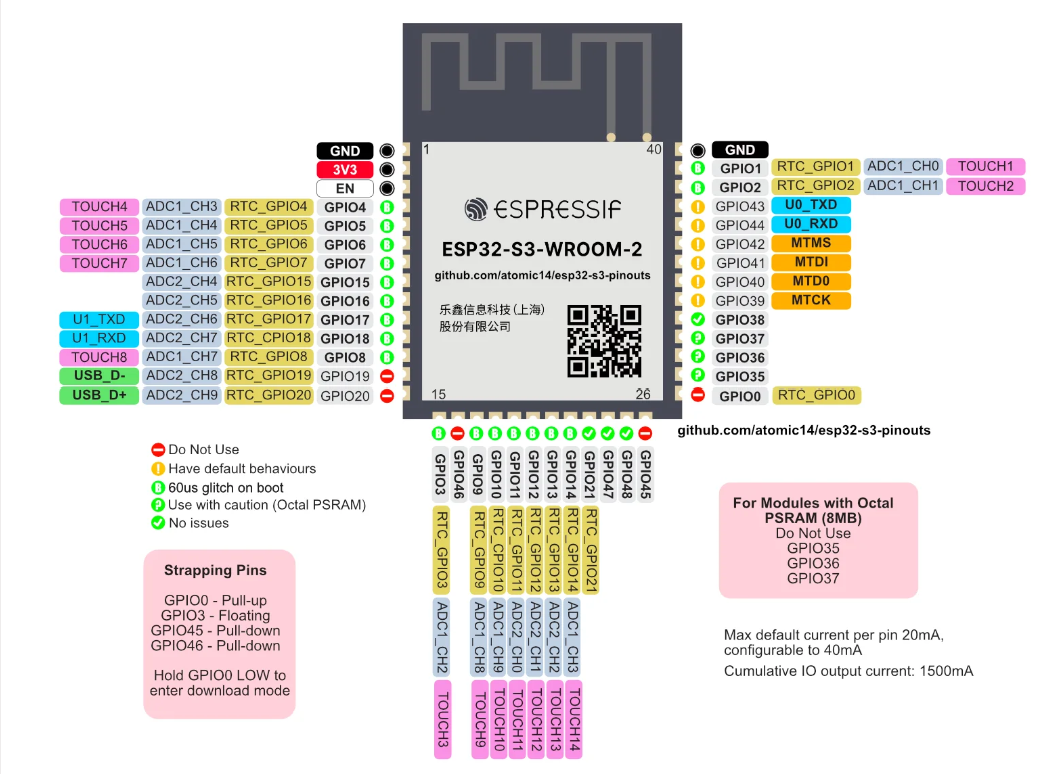
\includegraphics[width=1\textwidth]{Esp32.png}
  \caption{Rozkład pinów mikrokontrolera ESP32-S3\cite{st:esp32-pin}}
\end{figure}

\subsection{Zasilanie}
Według dokumentacji producenta, ESP32-S3 może być zasilany napięciem od 3V do 3.6V, zalecane napięcie zasilania to 3.3V.
Jego maksymalny pobór prądu wynosi 340mA, jednak w praktyce jest on znacznie mniejszy, zależy to od wykorzystywanych funkcji i peryferiów.

Układ można wprowadzić w dwa tryby uśpienia:
\begin{itemize}
\item Light Sleep - pobór prądu wynosi około 240uA, w tym odłączany jest moduł WiFi a wszystkie piny GPIO są w stanie wysokiej impedancji.
\item Deep Sleep - pobór prądu wynosi około 8uA, jedynie zasilany jest moduł RTC, wszystkie inne funkcje są wyłączone.
\end{itemize}

\end{document}
